The framework of Reinforcement Learning (RL) is based on the sequential interaction between an agent and an environment during several episodes, and --- as many ideas in artificial intelligence --- is strongly inspired in biological models of learning~\cite{Sutton2018,AlgorithmsRLCsaba}.

At each time-step $\ell=0,\cdots,L$ of each episode $t=1,\cdots,T$, the agent observes its environment in a \textit{state} $s_{\ell}^{(t)}\in\cS$ and chooses an \textit{action} $a_\ell^{(t)}\in\cA$; as a consequence, the agent enjoys a \textit{reward} $r_{\ell+1}^{(t)}\in\cR$ and observes a new state of the environment, $s_{\ell+1}^{(t)}\in\cS$; here $\cS$, $\cA$ and $\cR$
stand for the sets of states, actions and rewards the agent may experience. Such reward serves as a classical conditioning to the agent, who needs to train its behaviour in order to acquire as much rewards as possible, in a similar way we reward our dogs with soome cheese if they sit after saying ```\textit{seu}''\footnote{\textit{Seu }is \textit{sit} in catalan.}. In this sense, one might steer the agent towards optimal desired behaviours which are actually unkown to the designer of the reinforcement learning scenario: while we have the free will to define states, actions, rewards and envionment dynamics, it is highly unlikely that optimal behaviours that lead to high-rewards are known beforehand. This is the spirit of tackling open problems in science with reinforcement learning algorithms, where unknown solutions can readily be found by letting the sequential interaction to evolve over several episodes.

The environment is usually modeled to be Markovian: its dynamics is completely determined by the last time-step via the transition function $\tau(s',r|s,a)$, \textit{i.e.}, the conditional probability of ending up in a state $s'$ and conferring a reward $r$, given that the previous state was $s$ and the agent took an action $a$; the next future states accessible from $s$ are thus restricted to $\cS(s) = \{ s' : \tau(s'| s) \neq 0 \} \subseteq \cS$.

In general, the agent does not have control of nor access to the transition function, but it will influence the dynamics of the environment by choosing actions according to an interaction \textit{policy} $\pi(a|s)$, i.e., the conditional probability of performing an action $a$ when the observed environment's state is $s$; hence the available actions at a given state may be restricted to a subset $\cA(s) \subseteq \cA$. This setting is usually known as a Markov decision process (MDP).

The agent's objective is to interact with the environment through an \textit{optimal policy} $\pi^{*}$, for which the total reward acquired during an episode is as high as possible. In the dog-training case, this means getting as much cheese as possible, implying correctly execution of all the tricks. To achieve such goal, a \textit{value function} is assigned to each state and optimized over all possible policies, as explained in Sec.~\ref{ssec:1_rl_seqDec}.

\begin{figure}\label{fig:rldep}
\centering
    \begin{subfigure}[t!]{.49\textwidth}
        \centering
        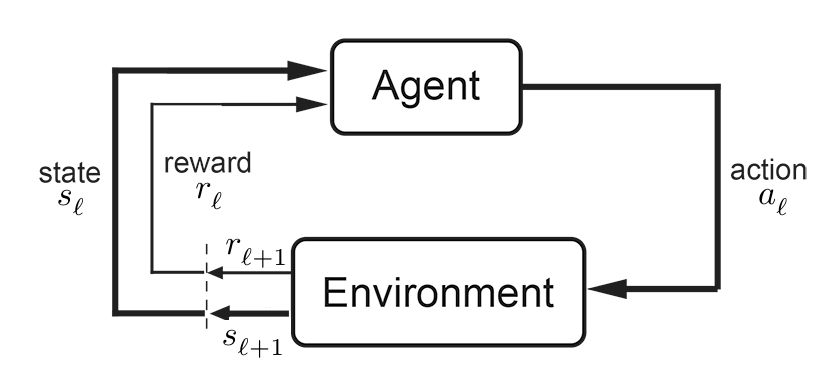
\includegraphics[width=1.\textwidth]{Figures/1rlintro/RL_papernotation.png}
    \end{subfigure}
    \hfill
    \begin{subfigure}[t!]{.49\textwidth}
        \centering
        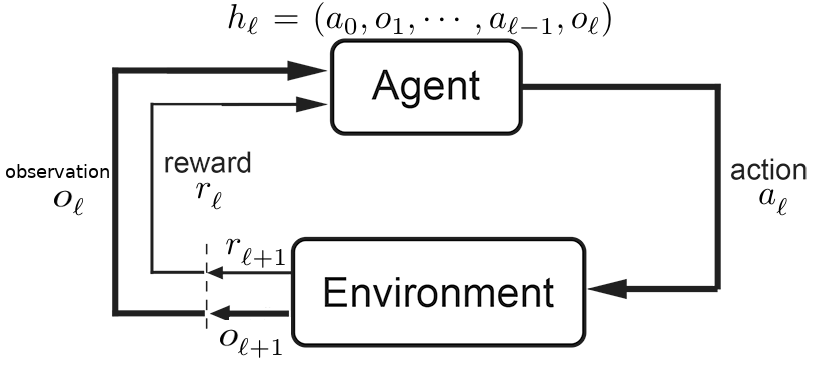
\includegraphics[width=1.\textwidth]{Figures/1rlintro/RL_papernotation_PO.png}
    \end{subfigure}
\caption{We depict the interaction with agent and environment in fully (left) and partially observable (right) cases.}
\end{figure}

The Markov assumption is justified whenever the agent's observations provide a complete description of the state of the environment $s_{\ell}$. However, in general this is not the case, and the agent has only access to \textit{partial observations} $o_{\ell}\in\cO$ at each time-step. This leads the agent to define its own state, \textit{e.g.} agent's state. While in the fully observable case agent's and environment's states coincide, in partially-observable environments the agent can only rely in such partial observations in order to learn. These observations would not allow to determine the dynamics even if $\tau$ was known, and they are generated from the current (environment) state and the previous interaction history (\textit{e.g.} actions performed, observations acquired and environments' states). In RL literature this is known as a partially-observable MDP (POMDP) and developing methods to solve it efficiently constitutes an active area of research~\cite{Singh1994,Mnih2013,Shani2013,Egorov2015,Zhu2018}; the problem is usually tackled by first reducing it to an effective MDP. The most straightforward approach is to define an effective state that contains all the past history of observations and actions up to a given time-step, \textit{i.e.}, $h_{\ell}=(a_0,o_{1},\cdots,a_{\ell-1},o_\ell)$. In this way, the dynamics observed by the agent can always be described by an effective MDP with transition function $\tau(h',r|h,a)$, which is unknown to the agent and determined by the underlying environmental transition function. We will choose such approach when framing quantum-state discrimination as reinforcement learning problem in Chapter~\ref{chapter:RLCOH}.

In order to gain some intuition on both the reinforcement learning problem and its difficulty, it is instructive to revist bandit problem. Such problem is a simplified version of the reinforcement learning setting, that yet captures many of the challenges underlying model-free learning frameworks. After discussing about bandits, we move to define value functions and study their associated Bellman equations in Sec.~\ref{ssec:1_rl_seqDec}, whereas in Sec.~\ref{ssec:1_rl_qlearning} we introduce the Q-learning algorithm, used to learn optimal policies in model-free settings. We finally comment on model-aware approaches such as dynammic programming in Sec.~\cite{ssec:1_rl_dp}.% and close this chapter with a discussion in Sec.~\cite{ssec:1_rl_discussion}
